\documentclass{article}
\usepackage{tikz}
\usepackage{amsmath}

\begin{document}

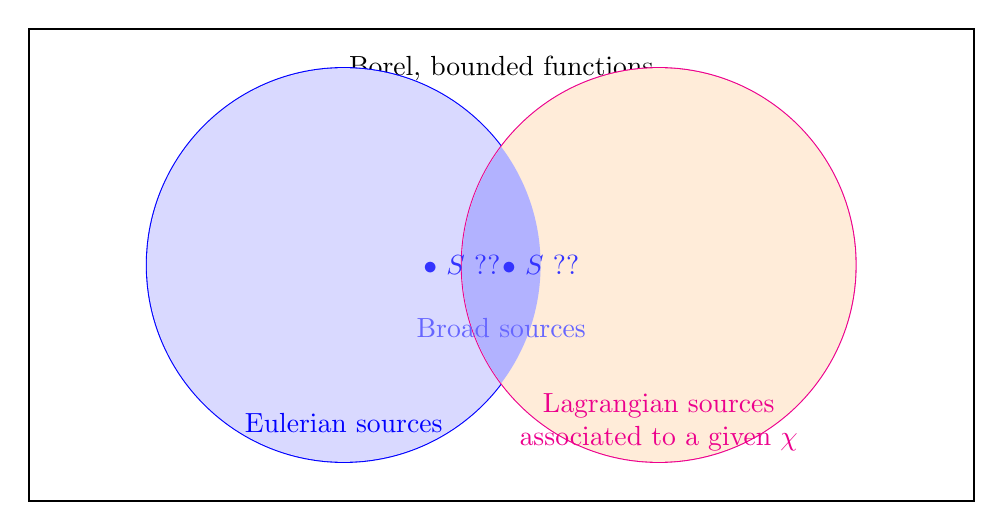
\begin{tikzpicture}[scale=1.0]
    % Draw the outer rectangle
    \draw [thick] (0,0) rectangle (12,6);
    
    % Add the title
    \node at (6,5.5) {Borel, bounded functions};
    
    % Draw the Eulerian sources circle
    \draw [blue, thick] (4,3) circle (2.5);
    \fill [blue!15] (4,3) circle (2.5);
    \node [blue] at (4,1) {Eulerian sources};
    
    % Draw the Lagrangian sources circle
    \draw [magenta, thick] (8,3) circle (2.5);
    \fill [orange!15] (8,3) circle (2.5);
    \node [magenta, align=center] at (8,1) {Lagrangian sources\\associated to a given $\chi$};
    
    % Draw the intersection (Broad sources)
    \begin{scope}
        \clip (4,3) circle (2.5);
        \fill [blue!30] (8,3) circle (2.5);
    \end{scope}
    
    % Add the "Broad sources" label
    \node [blue!60] at (6,2.2) {Broad sources};
    
    % Add the question marks in the intersection
    \node [blue!80] at (5.5,3) {$\bullet$ $S$ ??};
    \node [blue!80] at (6.5,3) {$\bullet$ $S$ ??};
    
\end{tikzpicture}

\end{document}